% !Mode:: "TeX:UTF-8"
% !TEX program = xelatex

\def\usewhat{xelatex}                               
\documentclass[12pt,openany,oneside, super]{ctexbook} %%super 将参考文献改为上标
                                                     % 本科生毕业论文通常采用单页排版
% !Mode:: "TeX:UTF-8"
%  Authors: 张井   Jing Zhang: prayever@gmail.com     天津大学2010级管理与经济学部信息管理与信息系统专业硕士生
%           余蓝涛 Lantao Yu: lantaoyu1991@gmail.com  天津大学2008级精密仪器与光电子工程学院测控技术与仪器专业本科生

%%%%%%%%%% Package %%%%%%%%%%%%
\usepackage{xeCJK}
\usepackage{fontspec}
\usepackage{CJK}
\usepackage{lmodern}
\usepackage[T1]{fontenc}
\usepackage{graphicx}                       % 支持插图处理
%\usepackage{caption}
\usepackage[a4paper,text={146.4true mm,239.2 true mm},top= 26.2true mm,left=31.8 true mm,head=6true mm,headsep=6.5true mm,foot=16.5true mm]{geometry}
                                            % 支持版面尺寸设置
\usepackage[squaren]{SIunits}               % 支持国际标准单位

\usepackage{titlesec}                       % 控制标题的宏包
\usepackage{titletoc}                       % 控制目录的宏包
\usepackage{fancyhdr}                       % fancyhdr宏包 支持页眉和页脚的相关定义
%\usepackage{ctex}                     % 支持中文显示
\usepackage{CJKpunct}                       % 精细调整中文的标点符号
\usepackage{color}                          % 支持彩色
\usepackage{amsmath}                        % AMSLaTeX宏包 用来排出更加漂亮的公式
\usepackage{amssymb}                        % 数学符号生成命令
\usepackage[below]{placeins}    %允许上一个section的浮动图形出现在下一个section的开始部分,还提供\FloatBarrier命令,使所有未处理的浮动图形立即被处理
\usepackage{multirow}                       % 使用Multirow宏包,使得表格可以合并多个row格
\usepackage{booktabs}                       % 表格,横的粗线;\specialrule{1pt}{0pt}{0pt}
\usepackage{longtable}                      % 支持跨页的表格。
\usepackage{tabularx}                       % 自动设置表格的列宽
\usepackage{subfigure}                      % 支持子图 %centerlast 设置最后一行是否居中
\usepackage[subfigure]{ccaption}            % 支持子图的中文标题
\usepackage[sort&compress,numbers]{natbib}  % 支持引用缩写的宏包
\usepackage{enumitem}                       % 使用enumitem宏包,改变列表项的格式
\usepackage{calc}                           % 长度可以用+ - * / 进行计算
\usepackage{txfonts}                        % 字体宏包
\usepackage{bm}                             % 处理数学公式中的黑斜体的宏包
\usepackage[amsmath,thmmarks,hyperref]{ntheorem}  % 定理类环境宏包,其中 amsmath 选项用来兼容 AMS LaTeX 的宏包
\usepackage{CJKnumb}                        % 提供将阿拉伯数字转换成中文数字的命令
\usepackage{indentfirst}                    % 首行缩进宏包
\usepackage{CJKutf8}                        % 用在UTF8编码环境下,它可以自动调用CJK,同时针对UTF8编码作了设置
\usepackage[numbers,sort&compress]{natbib} %%%参考文献多个引用中间用-连接
%\usepackage{hypbmsec}                      % 用来控制书签中标题显示内容
\newcommand{\tabincell}[2]{\begin{tabular}{@{}#1@{}}#2\end{tabular}}
\usepackage{xcolor}
%支持代码环境
\usepackage{listings}
\lstset{numbers=left,
language=[ANSI]{C},
numberstyle=\tiny,
extendedchars=false,
showstringspaces=false,
breakatwhitespace=false,
breaklines=true,
captionpos=b,
keywordstyle=\color{blue!70},
commentstyle=\color{red!50!green!50!blue!50},
frame=shadowbox,
rulesepcolor=\color{red!20!green!20!blue!20}
}
%支持算法环境
\usepackage[boxed,ruled,lined,linesnumbered]{algorithm2e}
\renewcommand{\algorithmcfname}{算法}
\SetAlFnt{\it}
%\usepackage{algorithm}
%\usepackage{algpseudocode}
%\usepackage{algorithmic}
%\usepackage{algpseudocode}
%\usepackage{algorithm}
%\usepackage[noend]{algpseudocode}

\usepackage{array}
\newcommand{\PreserveBackslash}[1]{\let\temp=\\#1\let\\=\temp}
\newcolumntype{C}[1]{>{\PreserveBackslash\centering}p{#1}}
\newcolumntype{R}[1]{>{\PreserveBackslash\raggedleft}p{#1}}
\newcolumntype{L}[1]{>{\PreserveBackslash\raggedright}p{#1}}

\def\atemp{xelatex}\ifx\atemp\usewhat
\usepackage{pdfpages}
\usepackage[unicode,
            pdfstartview=FitH,
            bookmarksnumbered=true,
            bookmarksopen=true,
            colorlinks=false,
            pdfborder={0 0 1},
            citecolor=blue,
            linkcolor=red,
            anchorcolor=green,
            urlcolor=blue,
            breaklinks=true
            ]{hyperref}
\fi
							% 定义本文所使用宏包
\graphicspath{figures/}							% 定义所有的图像文件在 figures 子目录下

\begin{document}								% 开始全文
% !Mode:: "TeX:UTF-8"
%  Authors: 张井   Jing Zhang: prayever@gmail.com     天津大学2010级管理与经济学部信息管理与信息系统专业硕士生
%           余蓝涛 Lantao Yu: lantaoyu1991@gmail.com  天津大学2008级精密仪器与光电子工程学院测控技术与仪器专业本科生
%			赵宇阳 Yuyang Zhao: yuyangzhao@outlook.com 天津大学2016级求是学部电子信息工程本科生

%%%%%%%%%%%%%%%%% Fonts Definition and Basics %%%%%%%%%%%%%%%%%
\setCJKfamilyfont{黑体}{SimHei} %{Noto Sans CJK SC} %{SimHei}
\setCJKfamilyfont{粗黑体}[Path=fonts/]{SourceHanSansSC-Medium.otf}%{SimHei} %{Noto Sans CJK SC} %{SimHei}
\setCJKfamilyfont{宋体}{SimSun}
\setCJKfamilyfont{粗宋体}[Path=fonts/]{SourceHanSerifSC-SemiBold.otf}
\newcommand{\hei}{\CJKfamily{黑体}}
\newcommand{\song}{\CJKfamily{宋体}}
\newcommand{\bfhei}{\CJKfamily{粗黑体}}
\newcommand{\bfsong}{\CJKfamily{粗宋体}}
\newcommand{\yihao}{\fontsize{26pt}{26pt}\selectfont}       % 一号, 单倍行距
\newcommand{\xiaoyi}{\fontsize{24pt}{24pt}\selectfont}      % 小一, 单倍行距
\newcommand{\erhao}{\fontsize{22pt}{1.25\baselineskip}\selectfont}       % 二号, 1.25倍行距
\newcommand{\xiaoer}{\fontsize{18pt}{18pt}\selectfont}      % 小二, 单倍行距
\newcommand{\sanhao}{\fontsize{16pt}{16pt}\selectfont}      % 三号, 单倍行距
\newcommand{\xiaosan}{\fontsize{15pt}{15pt}\selectfont}     % 小三, 单倍行距
\newcommand{\sihao}{\fontsize{14pt}{14pt}\selectfont}       % 四号, 单倍行距
\newcommand{\xiaosi}{\fontsize{12pt}{12pt}\selectfont}      % 小四, 单倍行距
\newcommand{\wuhao}{\fontsize{10.5pt}{10.5pt}\selectfont}   % 五号, 单倍行距
\newcommand{\xiaowu}{\fontsize{9pt}{9pt}\selectfont}        % 小五, 单倍行距

%\CJKtilde  % 重新定义了波浪符~的意义
% JUST DON'T USE CJK
% 使用 ctexbook 之后已无必要
\newcommand\prechaptername{第}
\newcommand\postchaptername{章}

\punctstyle{hangmobanjiao}             % 调整中文字符的表示,行内占一个字符宽度,行尾占半个字符宽度

% 调整罗列环境的布局
\setitemize{leftmargin=3em,itemsep=0em,partopsep=0em,parsep=0em,topsep=-0em}
\setenumerate{leftmargin=3em,itemsep=0em,partopsep=0em,parsep=0em,topsep=0em}

% 避免宏包 hyperref 和 arydshln 不兼容带来的目录链接失效的问题。
\def\temp{\relax}
\let\temp\addcontentsline
\gdef\addcontentsline{\phantomsection\temp}

% 自定义项目列表标签及格式 \begin{publist} 列表项 \end{publist}
\newcounter{pubctr} %自定义新计数器
\newenvironment{publist}{%%%%%定义新环境
\begin{list}{[\arabic{pubctr}]} %%标签格式
    {
     \usecounter{pubctr}
     \setlength{\leftmargin}{2.5em}   % 左边界 \leftmargin =\itemindent + \labelwidth + \labelsep
     \setlength{\itemindent}{0em}     % 标号缩进量
     \setlength{\labelsep}{1em}       % 标号和列表项之间的距离,默认0.5em
     \setlength{\rightmargin}{0em}    % 右边界
     \setlength{\topsep}{0ex}         % 列表到上下文的垂直距离
     \setlength{\parsep}{0ex}         % 段落间距
     \setlength{\itemsep}{0ex}        % 标签间距
     \setlength{\listparindent}{0pt}  % 段落缩进量
    }}
{\end{list}}

\makeatletter
\renewcommand\normalsize{
  \@setfontsize\normalsize{12pt}{12pt} % 小四对应 12 pt
  \setlength\abovedisplayskip{4pt}
  \setlength\abovedisplayshortskip{4pt}
  \setlength\belowdisplayskip{\abovedisplayskip}
  \setlength\belowdisplayshortskip{\abovedisplayshortskip}
  \let\@listi\@listI}
\def\defaultfont{\renewcommand{\baselinestretch}{1.63}\normalsize\selectfont} % 设置行距

\renewcommand{\CJKglue}{\hskip -0.1 pt plus 0.08\baselineskip} % 控制字间距,使每行 34 个汉字
\makeatother

%%%%%%%%%%%%% Contents %%%%%%%%%%%%%%%%%
\renewcommand{\contentsname}{目\qquad 录}
\setcounter{tocdepth}{2} % 控制目录深度
% 使用 ctexbook 之后已无必要
%\titlecontents{chapter}[2em]{\vspace{.5\baselineskip}\xiaosan\song}
             %{\prechaptername\CJKnumber{\thecontentslabel}\postchaptername\qquad}{}
             %{\hspace{.5em}\titlerule*[10pt]{$\cdot$}\sihao\contentspage}
\titlecontents{chapter}[2em]{\vspace{.25\baselineskip}\xiaosi\song}
             {\thecontentslabel\!\!\qquad}{}
             {\titlerule*[5pt]{$\cdot$}\xiaosi\contentspage}
\titlecontents{section}[3em]{\vspace{.25\baselineskip}\xiaosi\song}
             {\thecontentslabel\quad}{}
             {\titlerule*[5pt]{$\cdot$}\xiaosi\contentspage}
\titlecontents{subsection}[4em]{\vspace{.25\baselineskip}\xiaosi\song}
             {\thecontentslabel\quad}{}
             {\titlerule*[5pt]{$\cdot$}\xiaosi\contentspage}

%%%%%%%%%% Chapter and Section %%%%%%%%%%%%%
\setcounter{secnumdepth}{4}
\setlength{\parindent}{2em}
\renewcommand{\chaptername}{\prechaptername\CJKnumber{\thechapter}\postchaptername}
\titleformat{\chapter}{\centering\xiaosan\hei}{\chaptername}{2em}{}
\titlespacing{\chapter}{0pt}{0.1\baselineskip}{0.8\baselineskip}
\titleformat{\section}{\sihao\hei}{\thesection}{1em}{}
\titlespacing{\section}{0pt}{0.15\baselineskip}{0.25\baselineskip}
\titleformat{\subsection}{\sihao\hei}{\thesubsection}{1em}{}
\titlespacing{\subsection}{0pt}{0.1\baselineskip}{0.3\baselineskip}
\titleformat{\subsubsection}{\sihao\hei}{\thesubsubsection}{1em}{}
\titlespacing{\subsubsection}{0pt}{0.05\baselineskip}{0.1\baselineskip}

\newcommand{\trtitle}[1]{\vspace{12pt}\begin{center}{\xiaoer\hei\bf #1}\end{center}}
\newcommand{\trabs}[1]{\vspace{6pt}{\begin{center}{\xiaosan\hei #1}\end{center}}}
\newcommand{\trchapter}[1]{\vspace{6pt}{\raggedright\xiaosan\hei #1}}%%\newline}
\newcommand{\trsection}[1]{\vspace{4pt}{\raggedright\sihao\hei #1}}%%%\newline}
\newcommand{\trsubsection}[1]{\vspace{2pt}{\raggedright\sihao\hei\it #1}}%%%\newline}

%%%%%%%%%% Table, Figure and Equation %%%%%%%%%%%%%%%%%
\renewcommand{\tablename}{表}                                     % 插表题头
\renewcommand{\figurename}{图}                                    % 插图题头
\renewcommand{\thefigure}{\arabic{chapter}-\arabic{figure}}       % 使图编号为 7-1 的格式 %\protect{~}
\renewcommand{\thesubfigure}{\alph{subfigure})}                   % 使子图编号为 a) 的格式
\renewcommand{\thesubtable}{(\alph{subtable})}                    % 使子表编号为 (a) 的格式
\renewcommand{\thetable}{\arabic{chapter}-\arabic{table}}         % 使表编号为 7-1 的格式
\renewcommand{\theequation}{\arabic{chapter}-\arabic{equation}}   % 使公式编号为 7-1 的格式
\newcommand{\ud}{\mathrm{d}}

%%%%%% 定制浮动图形和表格标题样式 %%%%%%
\makeatletter
\long\def\@makecaption#1#2{
   \vskip\abovecaptionskip
   \sbox\@tempboxa{\centering\wuhao\song{#1\qquad #2} }
   \ifdim \wd\@tempboxa >\hsize
%     \centering\wuhao\song{#1\qquad #2} \par
     \wuhao\song{#1\quad #2} \par
   \else
     \global \@minipagefalse
     \hb@xt@\hsize{\hfil\box\@tempboxa\hfil}
   \fi
   \vskip\belowcaptionskip\vspace{8pt}}
\makeatother
\captiondelim{~~~~} %用来控制longtable表头分隔符

%%%%%%%%%% Theorem Environment %%%%%%%%%%%%%%%%%
\theoremstyle{plain}
\theorembodyfont{\song\rmfamily}
\theoremheaderfont{\hei\rmfamily}
\newtheorem{theorem}{定理~}[chapter]
\newtheorem{lemma}{引理~}[chapter]
\newtheorem{axiom}{公理~}[chapter]
\newtheorem{proposition}{命题~}[chapter]
\newtheorem{prop}{性质~}[chapter]
\newtheorem{corollary}{推论~}[chapter]
\newtheorem{definition}{定义~}[chapter]
\newtheorem{conjecture}{猜想~}[chapter]
\newtheorem{example}{例~}[chapter]
\newtheorem{remark}{注~}[chapter]
%\newtheorem{algorithm}{算法~}[chapter]
\newenvironment{proof}{\noindent{\hei 证明:}}{\hfill $ \square $ \vskip 4mm}
\theoremsymbol{$\square$}

%%%%%%%%%% Page: number, header and footer  %%%%%%%%%%%%%%%%%

%\frontmatter 或 \pagenumbering{roman}
%\mainmatter 或 \pagenumbering{arabic}
\makeatletter
\renewcommand\frontmatter{\clearpage
  \@mainmatterfalse
  }
\makeatother

%%%%%%%%%%% Code: Listings from MCM Template %%%%%%%%%%%%

\definecolor{grey}{rgb}{0.8,0.8,0.8}
\definecolor{darkgreen}{rgb}{0,0.3,0}
\definecolor{darkblue}{rgb}{0,0,0.3}
\def\lstbasicfont{\fontfamily{pcr}\selectfont\footnotesize}
\lstset{%
% indexing
   % numbers=left,
   % numberstyle=\small,%
% character display
    showstringspaces=false,
    showspaces=false,%
    tabsize=4,%
% style
    frame=lines,%
    basicstyle={\footnotesize\lstbasicfont},%
    keywordstyle=\color{darkblue}\bfseries,%
    identifierstyle=,%
    commentstyle=\color{darkgreen},%\itshape,%
    stringstyle=\color{black}%
}
\lstloadlanguages{C,C++,Java,Matlab,Mathematica,Python}

%%%%%%%%%%%% References %%%%%%%%%%%%%%%%%

\makeatletter
\renewenvironment{thebibliography}[1]{
   \wuhao
   \list{\@biblabel{\@arabic\c@enumiv}}
        {\renewcommand{\makelabel}[1]{##1\hfill}
         \settowidth\labelwidth{0 cm}
         \setlength{\labelsep}{0pt}
         \setlength{\itemindent}{0pt}
         \setlength{\leftmargin}{\labelwidth+\labelsep}
         \addtolength{\itemsep}{-0.7em}
         \usecounter{enumiv}
         \let\p@enumiv\@empty
         \renewcommand\theenumiv{\@arabic\c@enumiv}}
    \sloppy\frenchspacing
    \clubpenalty4000
    \@clubpenalty \clubpenalty
    \widowpenalty4000
    \interlinepenalty4000
    \sfcode`\.\@m}
   {\def\@noitemerr
     {\@latex@warning{Empty 'thebibliography' environment}}
    \endlist\frenchspacing}
\makeatother

\addtolength{\bibsep}{-0.5em}     % 缩小参考文献间的垂直间距
\setlength{\bibhang}{2em}         % 每个条目自第二行起缩进的距离

% 参考文献引用作为上标出现
\newcommand{\citeup}[1]{\textsuperscript{\cite{#1}}}

%%%%%%%%%%%% Cover %%%%%%%%%%%%%%%%%
% 封面、摘要、版权、致谢格式定义
\makeatletter
\def\ctitle#1{\def\@ctitle{#1}}\def\@ctitle{}
\def\cdegree#1{\def\@cdegree{#1}}\def\@cdegree{}
\def\caffil#1{\def\@caffil{#1}}\def\@caffil{}
\def\csubject#1{\def\@csubject{#1}}\def\@csubject{}
\def\cgrade#1{\def\@cgrade{#1}}\def\@cgrade{}
\def\cauthor#1{\def\@cauthor{#1}}\def\@cauthor{}
\def\cnumber#1{\def\@cnumber{#1}}\def\@cnumber{}
\def\csupervisor#1{\def\@csupervisor{#1}}\def\@csupervisor{}
\def\crank#1{\def\@crank{#1}}\def\@crank{}
\def\cdate#1{\def\@cdate{#1}}\def\@cdate{}
\long\def\cindependent#1{\long\def\@cindependent{#1}}\long\def\@cindependent{}
\long\def\cabstract#1{\long\def\@cabstract{#1}}\long\def\@cabstract{}
\long\def\eabstract#1{\long\def\@eabstract{#1}}\long\def\@eabstract{}
\def\ckeywords#1{\def\@ckeywords{#1}}\def\@ckeywords{}
\def\ekeywords#1{\def\@ekeywords{#1}}\def\@ekeywords{}
\def\cheading#1{\def\@cheading{#1}}\def\@cheading{}


\pagestyle{fancy}
\fancyhf{}
\fancyhead[C]{\song\wuhao \@cheading}  % 页眉显示天津大学 20XX 届本科生毕业论文
\fancyfoot[C]{\song\xiaowu ~\thepage~}
\newlength{\@title@width}

%%%%%%%%%%%%%%%%%%%     Cover     %%%%%%%%%%%%%%%%%%%%%%%
\def\makecover{
   	\phantomsection
    \pdfbookmark[-1]{\@ctitle}{ctitle}

    \begin{titlepage}
      	\vspace*{31.5pt}
      	\begin{center}
  			\begin{figure}[h]
  				\centering
  				
\includegraphics[width=0.4\textwidth]{figures/tjuname}
  			\end{figure}
%  			\vspace*{21pt}
%  			\hei\erhao{\textbf{本科生毕业设计(论文)}}
%  			\vspace*{52.5pt}
			\bfhei\erhao{本科生毕业设计(论文)}
  			\vspace*{48pt}
  						
  			\begin{figure}[h]
  				\centering
  				
\includegraphics[width=0.4\textwidth]{figures/tjulogo}
  			\end{figure}
%  			\vspace*{42pt}
			\vspace*{5pt}
			\bfhei\sanhao{\textbf{题目:{\@ctitle}}}
			\vspace*{24pt}
			  			
  			\renewcommand\arraystretch{1.5}
  			\setlength{\@title@width}{5cm}{\bfsong\sanhao{
    			\begin{tabular}{lc}
      				学\qquad 院&	\underline{\makebox[\@title@width][c]{\@caffil}}	\\
      				专\qquad 业&	\underline{\makebox[\@title@width][c]{\@csubject}}	\\
      				年\qquad 级&	\underline{\makebox[\@title@width][c]{\@cgrade}}	\\
      				姓\qquad 名&	\underline{\makebox[\@title@width][c]{\@cauthor}} 	\\
      				学\qquad 号&	\underline{\makebox[\@title@width][c]{\@cnumber}} 	\\
      				指导教师   &	\underline{\makebox[\@title@width][c]{\@csupervisor}} \\
  				\end{tabular}
  			}}
  			\vspace*{21pt}

%			\song\sanhao{\textbf{\@cdate}}
		\end{center}
	\end{titlepage}
}
%%%%%%%%%%%%%%%%%%%   Independent  %%%%%%%%%%%%%%%%%%%%%%%
\def\makeindependent{
	\titleformat{\chapter}{\centering\erhao\bfsong}{\chaptername}{2em}{}
	
	\clearpage
	\markboth{独创性声明}{独创性声明}
	\pdfbookmark[0]{独创性声明}{cindependent}
	\chapter*{独创性声明}
	\song\sanhao\defaultfont
	\@cindependent
	\vspace{\baselineskip}
	\thispagestyle{empty}
}
%%%%%%%%%%%%%%%%%%%    Abstract    %%%%%%%%%%%%%%%%%%%%%%%
\def\makeabstract{
	\titleformat{\chapter}{\centering\erhao\bfsong}{\chaptername}{2em}{} %"摘要"二号宋体加粗居中

%%%%% Chinese Abstract %%%%%
	\clearpage
	\markboth{摘~要}{摘~要}
	\pdfbookmark[0]{摘~~要}{cabstract}
	\chapter*{摘\qquad 要}
	
	\song\defaultfont
	\@cabstract
	\vspace{\baselineskip}

	\hangafter=1\hangindent=55pt
	\noindent
	{\bfsong\sihao{关键词:}} \@ckeywords %%%%%跟原文空一行小四12pt
	\thispagestyle{plain}

%%%%% English Abstract %%%%%
	\clearpage
	\markboth{ABSTRACT}{ABSTRACT}
	\pdfbookmark[0]{ABSTRACT}{eabstract}
	\chapter*{\textbf{ABSTRACT}}
	
	\@eabstract
	\vspace{\baselineskip}

	\hangafter=1\hangindent=81pt\noindent %%这个hangindent是为了下一行同样在keywords后边
	{\textbf{KEY WORDS:}} \@ekeywords 
	\thispagestyle{plain}
}

%%%%%%%%%%%%%%%%%%%    Contents    %%%%%%%%%%%%%%%%%%%%%%%
\def\makecontents{
	\titleformat{\chapter}{\centering\xiaosan\hei}{\chaptername}{2em}{} %"目录"小三黑体居中

	\clearpage{\pagestyle{plain}\cleardoublepage}
	\pdfbookmark[0]{目~~录}{mulu}
	\tableofcontents                                     % 中文目录
	\fancypagestyle{plain}{
		\fancyhf{}
		\renewcommand{\headrulewidth}{0 pt}
		\fancyfoot[C]{\song\xiaowu~\thepage~}
	}
	\thispagestyle{plain}

	\mainmatter\defaultfont\sloppy\raggedbottom
	\makeatletter
	\fancypagestyle{plain}{                              % 设置开章页眉页脚风格
    	\fancyhf{}
    	\fancyhead[C]{\song\wuhao \@cheading}            % 首页页眉格式
    	\fancyfoot[C]{\song\xiaowu ~\thepage~}           % 首页页脚格式
    	\renewcommand{\headrulewidth}{0.5pt}
    	\renewcommand{\footrulewidth}{0pt}
	}
}

%%%%%%%%%%%%%%%%%%%   References   %%%%%%%%%%%%%%%%%%%%%%%
\def\makereferences{
	\titleformat{\chapter}{\centering\xiaosan\hei}{\chaptername}{2em}{} % "参考文献"小三黑体顶格
	\setlength{\baselineskip}{17pt}
	\setlength{\parskip}{3pt}
	\chapter*{\bibname}
	\defaultfont
	\bibliographystyle{references/ref.bst}
	\bibliography{references/ref}

	\phantomsection
	\markboth{参考文献}{参考文献}
	\addcontentsline{toc}{chapter}{参考文献}       % 参考文献加入到中文目录
	%\nocite{*}                                     % 若将此命令屏蔽掉,则未引用的文献不会出现在文后的参考文献中
}

\makeatother

							% 完成对论文各个部分格式的设置
\frontmatter									% 以下是论文导言部分,包括论文的封面,中英文摘要和中文目录
\fancypagestyle{plain}{
	\fancyhf{}
	\fancyhead[C]{\song\wuhao \@cheading}
	\renewcommand{\headrulewidth}{0 pt}
	\fancyfoot[C]{\song\xiaowu~\thepage~}
}

\makecontents
\setcounter{page}{1}
% !Mode:: "TeX:UTF-8"
\baselineskip=20pt
\cheading{天津大学~2020~届本科生毕业论文}      	% 设置正文的页眉,需要填上对应的毕业年份
\title{他改变了中国:江泽民传}    	% 论文名称
\author{作者}            					% 作者姓名
\email{email: yuyangzhao@outlook.com} %作者邮箱
%%%%%%%%%%%%%如果作者和邮箱过长,可以在format.tex文件中makecover部分取消注释
%\chapter*{中文翻译}
\makecover
\begin{abstract}
\par\setlength{\parindent}{2em} 中文摘要一般在~400~字以内,简要介绍毕业论文的研究目的、方法、结果和结论,语言力求精炼。中英文摘要均要有关键词,一般为~3~—~7~个。字体为小四号宋体,各关键词之间要有分号。英文摘要应与中文摘要相对应,字体为小四号~Times New Roman。
\end{abstract}

\section{第一节}
\subsection{第二级标题}
《他改变了中国:江泽民传》(如图~\ref{book}~所示)这本传记介绍了江泽民同志的人生历程,尤其是阐述和评价了江泽民同志担任中国主要领导人的10多年中创立的历史功绩。在着重于国事活动的同时,也广泛涉及家庭生活、业余爱好、人品风格等方方面面,多角度、多侧面地展现了传主的风采。

\begin{figure}[htbp!]
	\centering
	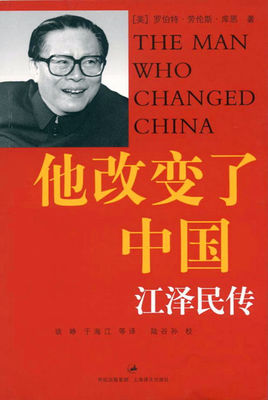
\includegraphics[width=0.5\textwidth]{figures/The_Man_Who_Changed_China.png}
	\caption{红宝书封面}\label{book}
	\vspace{-1em}
\end{figure}	

\begin{table}[htbp]
	\caption{长者用语对照表}\label{table}
	\vspace{0.5em}\centering\wuhao
	\begin{tabular}{ccccc}
		\toprule[1.5pt]
		原文 & 翻译 \\
		\midrule[1pt]
		吼哇 & 好啊 \\
		姿瓷 & 支持 \\
		姿势水平 & 知识水平 \\
		图样 & too young \\
		图森破 & too simple \\
		上台拿衣服 & sometimes naive \\
		识得唔识得啊 & 知道不知道啊 \\
		捉鸡 & 着急 \\
		这是坠吼滴 & 这是最好的 \\
		安格瑞 & angry \\
		一颗赛艇 & excited \\
		\bottomrule[1.5pt]
	\end{tabular}
	\vspace{\baselineskip}
\end{table}


\section{三件小事}
到了北京我干了这十几年也没有什么别的,大概三件事:

\begin{itemize}
	\item 一个,确立了社会主义市场经济;
	\item 第二个,把邓小平的理论列入了党章;
	\item 第三个,就是我们知道的“三个代表”。
\end{itemize}

\section{结论}
我们党要始终代表中国先进生产力的发展要求——就是党的理论、路线、纲领、方针、政策和各项工作,必须努力符合生产力发展的规律,体现不断推动社会生产力的解放和发展的要求,尤其要体现推动先进生产力发展的要求,通过发展生产力不断提高人民群众的生活水平;

我们党要始终代表中国先进文化的前进方向——就是党的理论、路线、纲领、方针、政策和各项工作,必须努力体现发展面向现代化、面向世界、面向未来的,民族的科学的大众的社会主义文化的要求,促进全民族思想道德素质和科学文化素质的不断提高,为我国经济发展和社会进步提供精神动力和智力支持;

我们党要始终代表中国最广大人民的根本利益——就是党的理论、路线、纲领、方针、政策和各项工作,必须坚持把人民的根本利益作为出发点和归宿,充分发挥人民群众的积极性主动性创造性,在社会不断发展进步的基础上,使人民群众不断获得切实的经济、政治、文化利益。


%%%%%%%%%%  参考文献  %%%%%%%%%%
\makereferences

%%%%%%%%%%    附录    %%%%%%%%%%
\clearpage
\end{document}									% 结束全文
